\documentclass[a4paper,10pt]{article}
\usepackage[utf8]{inputenc}
\usepackage[]{polski}
\usepackage{a4wide}
\usepackage{caption}
\usepackage{float}
\usepackage{amsthm}
\usepackage{graphicx}

\title{{\textbf{Pracownia z analizy numerycznej}}\\[1ex]
       {\Large Sprawozdanie do zadania \textbf{P2.20.}}\\[-1ex]
       {\Large Redukcja macierzy metodą Gaussa}\\
       {\large Prowadzący: dr Witold Karczewski}}
\author{Aleksander Balicki, \large nr indeksu: 220989\\
	Dominika Rogozińska, \large nr indeksu: 221094}

% Kropka po numerze paragrafu, podparagrafu itp. 
\makeatletter
	\renewcommand\@seccntformat[1]{\csname the#1\endcsname.\quad}
	\renewcommand\numberline[1]{#1.\hskip0.7em}
\makeatother

% Kropka po numerze tablicy, rysunku i ustawienie czcionki dla etykiety. 
\captionsetup{labelfont=sc,labelsep=period}

% Numeracja wzorów według paragrafu.
\renewcommand{\theequation}{\arabic{section}.\arabic{subsection}.\arabic{equation}}

% Zmiana nazwy figure "Rysunek" -> "Wykres"
\renewcommand{\figurename}{Wykres}

% Środowisko definition z numeracją
\newtheorem{definition}{Definicja}
\newtheorem{theorem}{Twierdzenie}


\date{Wrocław, \today r.}
\begin{document}
\maketitle

\section{Wstęp}
\setcounter{equation}{0}
Metodę Gaussa redukcji macierzy wykorzystuje się do rozwiązywania takich problemów jak znajdowanie macierzy odwrotnej, obliczanie rzędu macierzy, a także rozwiązywanie układów równań z wieloma niewiadomymi. Efektywność tej metody zależy od szczegółów implementacji i modyfikacji algorytmu oraz wskaźnika uwarunkowania macierzy. Poniżej zostały zaprezentowane wyniki otrzymane dla eliminacji Gaussa bez i z następującymi modyfikacjami: wybór największego(co do modułu) <<<<<<<<<reduktora>>>>>>>> z wiersza, z kolumny, z podmacierzy(wybór pełny). Badania zostały przeprowadzone dla kilku rodzajów macierzy: macierzy Hilberta, macierzy Pei, macierzy losowej z dominującą przekątną oraz macierzy oraz macierzy losowej, w ktorej większość elementów należy do przedziału $(-1,1)$, a kilka jest wybranych z zakresu $(-1000,1000)$.

\section{Definicje}
\begin{definition}
	Macierzą o wymiarach $m$ x $n$ (macierzą o $m$ wierszach i $n$ kolumnach), nad ciałem $K$ nazywamy każdą funkcję typu $\{1,\cdots,m\} \times \{1,\cdots,n\} \rightarrow K$.
\end{definition}
Interesują będą nas macierze o rozmiarach $n$ x $n$, które przedstawiają układy $n$ równań z $n$ niewiadomymi. Przykładowymi danymi do badań sposobów rozwiązania takich układów były macierze rzędu $n$, które są nieosobliwe, więc układy te zawsze mają rozwiązanie.
Macierz zapisujemy w następujący sposób:
\begin{center}
	$ \left[ \begin{array}{cccc}
		a_{1,1} & a_{1,2} & \cdots & a_{1,n}\\
		a_{2,1} & a_{2,2} & \cdots & a_{2,n}\\
		\vdots  &  \vdots &        & \vdots \\
		a_{m,1} & a_{m,2} & \cdots & a_{m,n}\\
	\end{array} \right] $
\end{center}

Weźmy przykładowy układ równań:
\begin{center}
$ \left \{ \begin{array}{ccccccccc}
		a_{1,1}x_{1} & + & a_{1,2}x_{2} & + & \cdots & + & a_{1,n}x_{n} & = & b_{1}\\
		a_{2,1}x_{1} & + & a_{2,2}x_{2} & + & \cdots & + & a_{2,n}x_{n} & = & b_{2}\\
		\vdots & & \vdots & &  \vdots & & \vdots & & \vdots \\
		a_{n,1}x_{1} & + & a_{n,2}x_{2} & + & \cdots & + & a_{n,n}x_{n} & = & b_{n}\\
       \end{array} \right. $
\end{center}
Z tym układem wiążemy macierz układu $A$ oraz wektor wyrazów wolnych $b$:
\begin{center}
$A = \left[ \begin{array}{ccccccccc}
		a_{1,1} & a_{1,2} & \cdots & a_{1,n}\\
		a_{2,1} & a_{2,2} & \cdots & a_{2,n}\\
		\vdots  &  \vdots &        & \vdots \\
		a_{n,1} & a_{n,2} & \cdots & a_{n,n}\\
       \end{array} \right] $
$b = \left[ \begin{array}{c}
		b_{1}\\
		b_{2}\\
		\vdots\\
		b_{n}\\
       \end{array} \right] $
\end{center}

\begin{definition}
	Macierzą Hilberta nazywamy macierz $n$ x $n$, w której\\
    \begin{center}
    $a_{i,j} = \frac{1}{i+j-1}$
    \end{center}
\end{definition}\\

\begin{definition}
	Macierzą Pei nazywamy macierz $n$ x $n$, w której\\
  \[
  a_{i,j} = \left\{
  \begin{array}{l l}
    1 \quad \text{ $i$ \neq $j$ }\\
    d \quad \text{ $i$ = $j$ }\\
  \end{array} \right.
  \]
    gdzie $d$ jest parametrem.
\end{definition}\\

\begin{definition}
    Macierzą o dominującej przekątnej nazywamy macierz, w której\\
    \begin{center}
    $ \bigwedge_{\substack{i}} 
        \sum_{\substack{{ j \neq i }}
            |a_{i,j}| \leq |a_{i,i}| $
    \end{center}
\end{definition}\\

%TODO: wskaźnik uwarunkowania

\begin{definition}
    Normę maksimum dla wektora $x = \left[ x_{1}, x_{2}, \cdots , x_{n} \right] $ definiujemy jako\\
    \begin{center}
        $ \|x\|_{\infty} = max \{|x_{i}| : i = 1, 2, \cdots , n \}$
    \end{center}
\end{definition}\\

Normy maksimum użyjemy jako wskaźnika numerycznej poprawności metody Gaussa, porównując wartości $ \| b - A \tilde{x} \|_{\infty}$ dla wszystkich prób.

\section{Metoda eliminacji Gaussa}
	Metoda ta została stworzona przez Carla Friedricha Gaussa. Daje ona algorytm do rozwiązania układu równań liniowych,
	obliczenia rzędu macierzy i znalezienia macierzy odwrotnej do danej. Algorytm składa się z 2 kroków, najpierw doprowadzamy
	macierz do postaci schodkowej, a następnie znajdujemy wynik układu poprzez podstawienie w tył(funkcja back substitution).
	W metodzie Gaussa stososuje się 3 operacje elementarne na wierszach macierzy. Te operacje to:
	\begin{enumerate}
		\item Zamiana kolejności wierszy
		\item Pomnożenie wszystkich wartości w wierszu przez niezerowy skalar $\lambda$
		\item Dodanie do dowolnego wiersza kombinacji liniowej pozostałych wierszy
	\end{enumerate}
	Operacje elementarne mają ciekawe własności, mianowicie:
	\begin{itemize}
		\item Nie zmieniają rzędu macierzy
		\item Dowolną macierz można za pomocą skończonej liczby kroków doprowadzić do macierzy w postaci schodkowej
	\end{itemize}
	\subsection{Metoda eliminacji Gaussa bez wyboru elementów głównych}%TODO
    \subsection{Metoda eliminacji Gaussa z wyborem elementów głownych z wiersza}%TODO
    \subsection{Metoda eliminacji Gaussa z wyborem elementów głównych z kolumny}%TODO
    \subsection{Metoda eliminacji Gaussa z pełnym wyborem elementów głównych(z podmacierzy)}%TODO
%tu się zaczyna Twoje stare
		Nasz algorytm zauważy zero na pozycji $Z_{1,1}$. Zamieni pierwszy wiersz z drugim. Uzna, że wartość $Z_{1,1}$ jest niezerowa i przejdzie
	do następnego kroku. W trakcie algorytmu wykona się dzielenie $45/0.0000000000001$. Wiemy, z \cite{SL}, że przy dzieleniu przez liczby bliskie zeru
	następuje utrata cyfr dokładnych wyniku. Algorytm zachowywałby się zdecydowanie lepiej, jeżeli dzielilibyśmy przez większą liczbę.
		Algorytm wyboru elementu głównego w kolumnie:
	\begin{verbatim}
		for k from 1 to N-1
		    znajdz wiersz, w którym jest maksymalna wartość |M[i,k]| dla wszystkich i > k
		    zamień wiersz z tą maksymalną wartością z k-tym wierszem
		    for i from k+1 to N
		        odejmij od i-tego wiersza k-ty wiersz (M[i,k]/M[k,k]) razy
		zwróć ilość niezerowych wierszy
	\end{verbatim}
	Można też szukać elementu o największym module w całej podmacierzy,
	wydłuża to czas obliczeń, ale poprawia własności numeryczne.
		Algorytm z wyborem pełnym:
	\begin{verbatim}
		for k from 1 to N-1
		    znajdz i,l takie, że |M[i,l]| jest maksymalne dla wszystkich i > k, l > k
		    zamień l-tą kolumnę z k-tą kolumną
		    zamień i-ty wiersze z k-tym wierszem
		    zamień wiersz z tą maksymalną wartością z k-tym wierszem
		    for i from k+1 to N
		        odejmij od i-tego wiersza k-ty wiersz (M[i,k]/M[k,k]) razy
		zwróć ilość niezerowych wierszy
	\end{verbatim}
%tu się kończy Twoje stare
\section{Program}
	Program testujący jest napisany w języku C++. Użyto typu podwójnej precyzji (double). Wyniki zostały zapisane jako plik z rozszerzeniem .csv, a następnie opracowane graficznie za pomocą programu gnuplot.
	
\section{Wyniki prób}
    \subsection{Macierz Hilberta}
        \begin{center}
            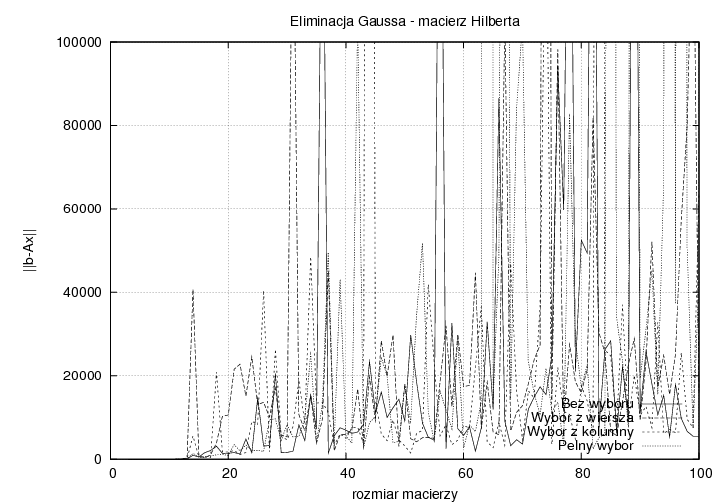
\includegraphics[width=140mm]{hilbert_plot.png}
        \end{center}
        Źle uwarunkowana, leci w kosmos. Wykres nie obejmuje całego zakresu.
    \subsection{Macierz Pei}
        \begin{center}
            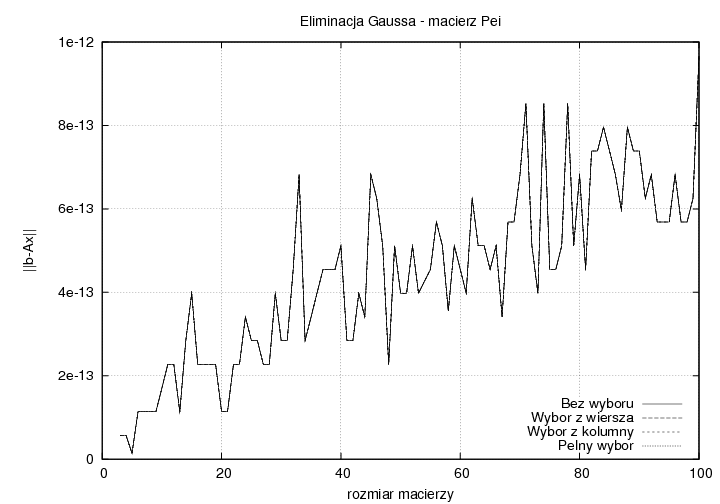
\includegraphics[width=140mm]{pei_plot.png}
        \end{center}
        Dobrze uwarunkowana, wygląda tak samo dla każdej modyfikacji algorytmu -> na przekątnej sa największe liczby i są równe.
    \subsection{Macierz z dominującą przekątną}
        \begin{center}
            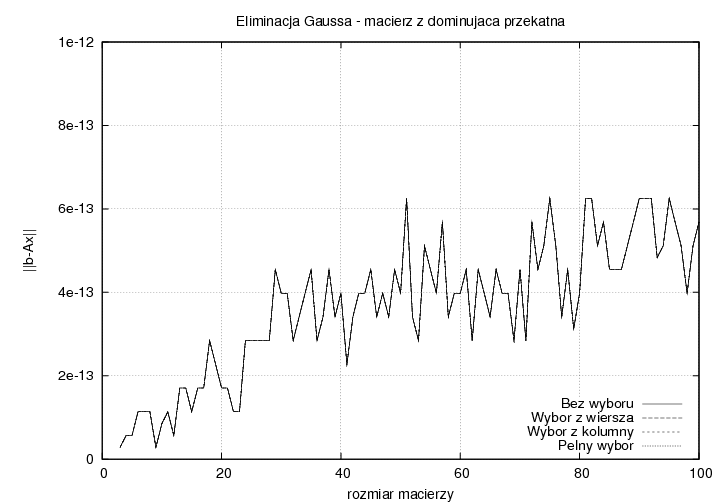
\includegraphics[width=140mm]{dominating_plot.png}
        \end{center}
        Dobrze uwarunkowana, dla metody bez modyfikacji i wyboru z wiersza(po którym zmieniamy kolumny) nie za dobrze, dla wyboru z kolumn i full lepiej i prawie tak samo.
    \subsection{Macierz losowa}
        \begin{center}
            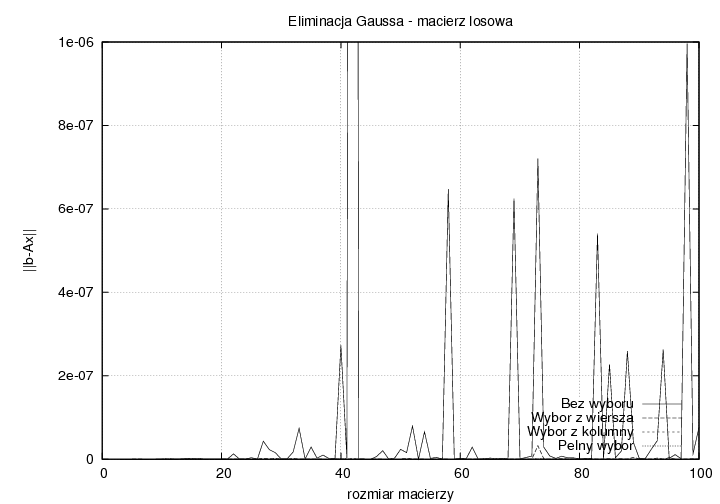
\includegraphics[width=140mm]{random_plot.png}
        \end{center}
        \begin{center}
            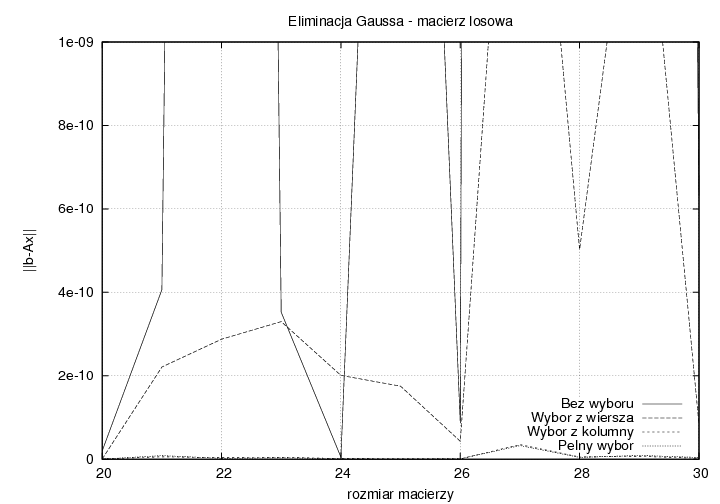
\includegraphics[width=140mm]{random_focus_plot.png}
        \end{center}

\section{Wnioski}
	
\begin{thebibliography}{9}
	\bibitem{EK} Notatki z wykładu Algebra Emanuela Kierońskiego
	\bibitem{SL} Notatki z wykładu Analiza Numeryczna Stanisława Lewanowicza
	\bibitem{KC} Kincaid David, Cheney Ward, Analiza numeryczna
	\bibitem{JJ} J. M. Jankowscy, Przegląd metod i algorytmów numerycznych
	\bibitem{Wa} http://wolframalpha.com/
	\bibitem{Wi} http://en.wikipedia.org/
	\bibitem{Mi} http://wazniak.mimuw.edu.pl/
\end{thebibliography}
\end{document}

